\section{Constructing the signed walk}\label{sec:construction}

We will encode the signed walk by one point in a convex body in a larger
coefficient space.  The body controls a contracted version of every prefix.
Its extra coordinates will be chosen so that their contributions exactly
restore the parts removed by the contractions.  This section states the two
analytic inputs and proves Theorem~\ref{thm:signing} from them.

\subsection{The two analytic inputs}

Let $D\subset\R^m$ be a nonempty bounded open convex set, and let $Q$ be a
positive definite diagonal $m\times m$ matrix.  Define its diagonal Dirichlet
energy by
\begin{equation}\label{eq:dirichlet-energy}
 \lambda_Q(D)=
 \inf_{0\ne g\in H^1_0(D)}
 \frac{\displaystyle\int_D\langle Q\nabla g,\nabla g\rangle\,dx}
      {\displaystyle\int_Dg^2\,dx}.
\end{equation}
Here $H^1_0(D)$ is the closure of $C_c^\infty(D)$ in the Sobolev norm, and
derivatives are weak derivatives.  This normalization corresponds to
Brownian motion with covariance rate $2Q$.  Central symmetry will always
mean symmetry about the origin.  Fix
\begin{equation}\label{eq:signing-constants}
 \kappa=\frac1{100},\qquad \delta=\frac14.
\end{equation}

Our first input turns small coordinate energies into signs while allowing a
bounded shift at each step.  The shifts may depend on previously assigned
coordinates.

\begin{proposition}[Signs with adaptive shifts]\label{prop:adaptive}
Let $K\subset\R^m$ be nonempty, bounded, open, convex and centrally
symmetric.  Suppose that
\begin{equation}\label{eq:all-diagonal-energy}
 \lambda_Q(K)\le\kappa^2\tr Q
 \quad\text{for every positive definite diagonal }Q.
\end{equation}
Let $j_1,\ldots,j_s$ be distinct elements of $\{1,\ldots,m\}$, and let
$q_i:\R^{i-1}\to[-\delta,\delta]$ be arbitrary functions, for
$1\le i\le s$.  There exist signs $\varepsilon_1,\ldots,\varepsilon_s$
such that the recursion
\[
 x^{(0)}=0,\qquad
 x^{(i)}=x^{(i-1)}+
 \bigl(q_i(x^{(i-1)}_{j_1},\ldots,x^{(i-1)}_{j_{i-1}})
       +\varepsilon_i\bigr)e_{j_i}
\]
has $x^{(s)}\in K$.  For $i=1$, the function $q_1$ has a one-point domain.
\end{proposition}

This is an existence statement; the choice of signs can depend on the whole
body $K$ and all the prescribed functions.  Its proof uses backward
transformations of $K$, followed by forward choices of the signs.

The second input supplies a body satisfying a uniform energy bound.  Its
linear maps retain a $d$-dimensional state and read one new coordinate at
each step.

\begin{proposition}[Energy of a filtered path body]\label{prop:filtered}
There are positive absolute constants $A_0,B_0,H_0$ with the following
property.  Let $d\ge1$ and $n\ge0$ be integers and put $m=d+n$.  For
$1\le t\le n$, let $C_t$ be an invertible real $d\times d$ matrix and let
$b_t\in\R^d$ satisfy
\[
 C_tC_t^T+b_tb_t^T=I_d.
\]
Define linear maps $R_t:\R^m\to\R^d$ by
\begin{equation}\label{eq:filter-recursion}
 R_0x=(x_1,\ldots,x_d),\qquad
 R_tx=C_tR_{t-1}x+b_tx_{d+t}\quad(1\le t\le n).
\end{equation}
Then the bounded open convex centrally symmetric set
\begin{equation}\label{eq:filtered-body}
 \mathcal D=
 \left\{x\in\R^m:
 \begin{array}{ll}
 |x_j|<B_0 & (1\le j\le m),\\
 \lVert R_tx\rVert_2<A_0\sqrt d & (0\le t\le n)
 \end{array}\right\}
\end{equation}
satisfies
\[
 \lambda_Q(\mathcal D)\le H_0\tr Q
 \quad\text{for every positive definite diagonal }Q.
\]
\end{proposition}

The constants are independent of the number of maps and of $Q$.  This
uniformity is essential: the application will use $n$ equal to the number
of vectors.  To compensate for the contractions, we will also impose linear
constraints on the coefficients.  The following estimate bounds their
additional energy cost; we prove it after completing the construction.

\begin{lemma}[Adding slabs]\label{lem:slab-energy}
Let $D\subset\R^m$ be bounded, nonempty, open, convex and centrally
symmetric.  Let $D_*>0$, $\delta>0$, and let $m_1,\ldots,m_n$ be real
rows of length $m$.  Set
\[
 K=(2D_*D)\cap\bigcap_{i=1}^n\{x:|m_i x|<\delta\}.
\]
For every positive definite diagonal $Q$,
\begin{equation}\label{eq:slab-energy}
 \lambda_Q(K)
 \le D_*^{-2}\lambda_Q(D)
     +\pi^2\delta^{-2}\sum_{i=1}^n m_iQm_i^T.
\end{equation}
\end{lemma}

\subsection{The filter, the shifts, and their cancellation}

We now prove the signed-prefix theorem from
Propositions~\ref{prop:adaptive} and~\ref{prop:filtered}.  Their proofs in the
remaining sections are independent of this application.

\begin{proof}[Proof of Theorem~\ref{thm:signing}]
Write the prescribed sequence as $v_1,\ldots,v_n\in\R^d$, with
$\lVert v_i\rVert_2\le1$.  The hypotheses give $d,n\ge1$.

\paragraph{The symmetric contractions.}
For a positive absolute $\sigma<1$, to be chosen below, set
\begin{equation}\label{eq:symmetric-filter}
 b_i=\sigma v_i,\qquad
 \eta_i=\frac1{1+\sqrt{1-\lVert b_i\rVert_2^2}},\qquad
 C_i=I-\eta_ib_ib_i^T.
\end{equation}
On the span of $b_i$, the matrix $C_i$ has eigenvalue
$\sqrt{1-\lVert b_i\rVert_2^2}$, and on its orthogonal complement it is the
identity.  This includes $b_i=0$, for which $\eta_i=1/2$ and $C_i=I$.
Consequently
\[
 C_i=(I-b_ib_i^T)^{1/2}=C_i^T\succ0,
 \qquad C_i^2+b_ib_i^T=I,
 \qquad \frac12\le\eta_i\le1.
\]
Use these matrices in~\eqref{eq:filter-recursion}, and let $\mathcal D$ be
the body in Proposition~\ref{prop:filtered}.

For $x\in\R^{d+n}$, let $x^0$ be obtained by setting its first $d$
coordinates to zero.  Define row vectors $m_i$ by
\begin{equation}\label{eq:predictor-rows}
 m_ix=\eta_i b_i^TR_{i-1}x^0.
\end{equation}
Each row $m_i$ is supported only on the noise coordinates
$d+1,\ldots,d+i-1$.  In particular it is unaffected by any coordinate
assigned at step $i$ or later.

\paragraph{The cost of the predictor constraints.}
Let $M$ be the matrix with rows $m_i$.  We claim that every column of $M$
has squared Euclidean norm at most $\sigma^2$.  Its initial $d$ columns are
zero.  For a noise coordinate $d+j$, follow its contribution to the state:
\[
 r_j=b_j,\qquad r_i=C_ir_{i-1}\quad(j<i\le n).
\]
The coefficient of that coordinate in $m_i$ is zero for $i\le j$, and is
$\eta_i b_i^Tr_{i-1}$ for $i>j$.  Symmetry of $C_i$ gives the exact loss
identity
\[
 \lVert r_{i-1}\rVert_2^2-\lVert r_i\rVert_2^2
 =(b_i^Tr_{i-1})^2.
\]
Thus the losses telescope:
\begin{equation}\label{eq:predictor-columns}
 \begin{aligned}
 \lVert Me_{d+j}\rVert_2^2
 &=\sum_{i=j+1}^n\eta_i^2(b_i^Tr_{i-1})^2\\
 &\le\sum_{i=j+1}^n
       \bigl(\lVert r_{i-1}\rVert_2^2-\lVert r_i\rVert_2^2\bigr)
 \le\lVert b_j\rVert_2^2\le\sigma^2.
 \end{aligned}
\end{equation}
In particular, for every positive definite diagonal $Q$,
\begin{equation}\label{eq:predictor-weighted-cost}
 \sum_{i=1}^n m_iQm_i^T
 =\sum_{j=1}^{d+n}Q_{jj}\lVert Me_j\rVert_2^2
 \le\sigma^2\tr Q.
\end{equation}

Choose an absolute dilation $D_*>0$ and define
\begin{equation}\label{eq:application-body}
 K=(2D_*\mathcal D)\cap
   \{x:|m_ix|<\delta\text{ for }1\le i\le n\}.
\end{equation}
This is a bounded open convex centrally symmetric set containing a
neighborhood of zero.  Lemma~\ref{lem:slab-energy},
Proposition~\ref{prop:filtered}, and~\eqref{eq:predictor-weighted-cost} give
\begin{equation}\label{eq:application-energy}
 \lambda_Q(K)
 \le\left(H_0D_*^{-2}+\pi^2\delta^{-2}\sigma^2\right)\tr Q.
\end{equation}
We can therefore fix, once and for all,
\begin{equation}\label{eq:absolute-parameters}
 D_*\ge\max\{1,\sqrt{2H_0}/\kappa\},\qquad
 \sigma=\min\{1/2,\kappa\delta/(\sqrt2\pi)\}.
\end{equation}
The same body $K$ then satisfies~\eqref{eq:all-diagonal-energy} for every
positive definite diagonal $Q$.  These choices are independent of $d$, $n$
and the vectors.

\paragraph{Choosing the coefficients.}
For $u\in\R$ write
$\operatorname{clip}_\delta(u)=\max\{-\delta,\min\{u,\delta\}\}$.
Apply Proposition~\ref{prop:adaptive} to the distinct axes
$e_{d+1},\ldots,e_{d+n}$.  At step $i$ prescribe the shift
\[
 q_i=\operatorname{clip}_\delta(m_ix^{(i-1)}).
\]
By the support of $m_i$, this is a function of the previously assigned
coordinates, as required.  The proposition supplies signs and a final point
$x=x^{(n)}\in K$.  Its first $d$ coordinates remain zero.  Also, coordinates
assigned before step $i$ never change afterward, so
\[
 m_ix^{(i-1)}=m_ix.
\]
The final membership $x\in K$ implies $|m_ix|<\delta$.  Hence each shift
was already within the permitted interval: clipping was inactive, and
\begin{equation}\label{eq:unclipped-coordinates}
 x_{d+i}=m_ix+\varepsilon_i
 =\eta_i b_i^TR_{i-1}x+\varepsilon_i.
\end{equation}
Here $x^0=x$ because the initial block is zero.  Clipping is used only to
make the application of Proposition~\ref{prop:adaptive} unconditional;
causality and the final constraints subsequently remove it.

Figure~\ref{fig:cancellation} illustrates the identity that completes the
construction.

\paragraph{Cancellation.}
For this single final coefficient vector, $R_0x=0$ and
\begin{align*}
 R_tx
 &=C_tR_{t-1}x+b_tx_{d+t}\\
 &=(I-\eta_tb_tb_t^T)R_{t-1}x
   +b_t(\eta_tb_t^TR_{t-1}x+\varepsilon_t)\\
 &=R_{t-1}x+\varepsilon_tb_t.
\end{align*}
Thus, simultaneously for every $0\le t\le n$,
\begin{equation}\label{eq:feedback-cancellation}
 R_tx=\sum_{i=1}^t\varepsilon_ib_i.
\end{equation}
Since $x\in2D_*\mathcal D$, all these states have norm less than
$2D_*A_0\sqrt d$.  Dividing~\eqref{eq:feedback-cancellation} by $\sigma$
proves Theorem~\ref{thm:signing} with the absolute constant
$C=2D_*A_0/\sigma$.
\end{proof}

\begin{figure}[htbp]
 \centering
 \resizebox{0.96\textwidth}{!}{%
 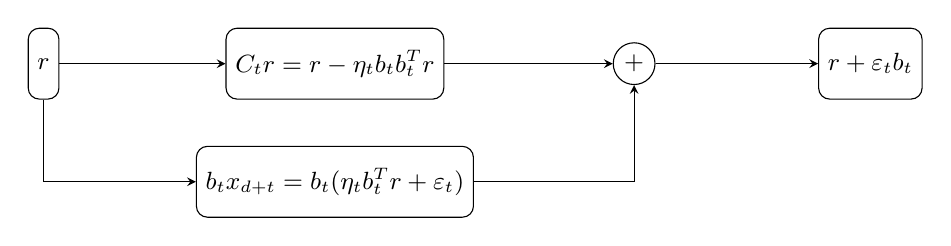
\begin{tikzpicture}[
   >=stealth,
   every node/.style={font=\small},
   state/.style={draw,rounded corners,align=center,minimum height=9mm}]
  \node[state] (r) at (0,0) {$r$};
  \node[state] (contract) at (3.7,0)
    {$C_tr=r-\eta_tb_tb_t^Tr$};
  \node[draw,circle,inner sep=2pt] (sum) at (7.5,0) {$+$};
  \node[state] (out) at (10.5,0) {$r+\varepsilon_tb_t$};
  \node[state] (incoming) at (3.7,-1.5)
    {$b_tx_{d+t}=b_t(\eta_tb_t^Tr+\varepsilon_t)$};
  \draw[->] (r) -- (contract);
  \draw[->] (contract) -- (sum);
  \draw[->] (sum) -- (out);
  \draw[->] (r.south) -- (0,-1.5) -- (incoming.west);
  \draw[->] (incoming.east) -- (7.5,-1.5) -- (sum.south);
 \end{tikzpicture}}
 \caption{For the final coefficient vector, put $r=R_{t-1}x$.
 The predictor term in the incoming coordinate restores exactly the
 component removed by $C_t$, leaving the signed increment
 $\varepsilon_tb_t$.}
 \label{fig:cancellation}
\end{figure}

\subsection{Brownian proofs of the slab bound}

We now prove Lemma~\ref{lem:slab-energy}, which bounded the cost of the
predictor constraints.  Brownian survival converts intersection with slabs
into an event to which Gaussian correlation applies.  The two Brownian
facts below will also be used in the remaining analytic arguments.

\begin{lemma}[Brownian survival rate]\label{lem:brownian-rate}
Let $D\subset\R^m$ be bounded, nonempty, open and convex, and let $Q$ be
positive definite and diagonal.  If $W$ is Brownian motion with covariance
rate $2Q$, started at $x\in D$, then
\begin{equation}\label{eq:brownian-rate}
 \lim_{T\to\infty}-\frac1T
 \log\mathbb P_x\{W(s)\in D\text{ for all }0\le s\le T\}
 =\lambda_Q(D).
\end{equation}
In particular, the starting point may be $0$ when $D$ is centrally
symmetric.
\end{lemma}

\begin{proof}
The generator of $W$ is $\tr(Q\nabla^2)$.  Let
$\tau_D=\inf\{s\ge0:W(s)\notin D\}$, and let
\[
 P_s^D h(x)=\mathbb E_x[h(W(s))\mathbf 1_{\{s<\tau_D\}}]
\]
be its killed semigroup.  The corresponding nonnegative self-adjoint
operator is the Dirichlet realization of $-\tr(Q\nabla^2)$, with form
$\int_D\nabla g^TQ\nabla g$ on $H_0^1(D)$.
These standard Dirichlet facts apply here because bounded convex domains
are connected and Lipschitz; see, for example,
\cite[Section~2 and Appendix~C]{DaviesSimon1984}, after the linear change
of coordinates for $Q$ and the time normalization above.
The killed representation can also be obtained first on smooth interior
domains and then by exhaustion: their compactly supported smooth
functions exhaust the form domain, while any continuous path remaining
in $D$ on a compact time interval has compact image in $D$.

Write $\lambda=\lambda_Q(D)$.  Compactness of
$H_0^1(D)\hookrightarrow L^2(D)$ and the spectral theorem give
$\lVert P_s^D\rVert_{2\to2}=e^{-s\lambda}$ and a first eigenfunction
$\varphi$ that can be chosen nonnegative by taking the absolute value
of a Rayleigh minimizer.  Interior elliptic regularity and the strong
maximum principle make $\varphi$ strictly positive at every point of $D$.
It is bounded: free heat
kernel domination and
$\varphi=e^\lambda P_1^D\varphi$ give this directly by
Cauchy--Schwarz.  Consequently,
\[
 e^{-T\lambda}\varphi(x)
 =P_T^D\varphi(x)
 \le \lVert\varphi\rVert_\infty\,
       \mathbb P_x\{\tau_D>T\}.
\]
For the reverse bound, let $p_Q$ denote the free heat kernel.  For $T\ge1$,
the semigroup property and free kernel domination yield
\begin{align*}
 \mathbb P_x\{\tau_D>T\}
 &\le \lVert p_Q(1,x,\cdot)\rVert_2
           \lVert P_{T-1}^D\mathbf 1_D\rVert_2\\
 &\le \lVert p_Q(1,x,\cdot)\rVert_2\,|D|^{1/2}
           e^{-(T-1)\lambda}.
\end{align*}
Both prefactors are finite for the fixed $D,Q,x$.
Taking logarithms and dividing by $T$ proves
\eqref{eq:brownian-rate}.  Finally, a nonempty open convex set symmetric
about $0$ contains $0$ as an interior point.
\end{proof}

We will use the following path form of Gaussian correlation.  Its
finite-grid proof also records how closed constraints are handled.

\begin{lemma}[Gaussian correlation for path constraints]
\label{lem:gaussian-path-correlation}
Let $X:[0,T]\to\R^m$ be a centered Gaussian process with continuous paths.
For $i=1,\ldots,r$, let $E_i$ be an event of the form
\[
 E_i=\bigcap_{j=1}^{r_i}
 \{A_{ij}X(s)\in K_{ij}\text{ for all }s\in I_{ij}\},
\]
where $A_{ij}$ is linear, $K_{ij}$ is a closed centrally symmetric convex
set in its target space, and $I_{ij}\subset[0,T]$ is a closed interval.
Then
\[
 \mathbb P\Bigl(\bigcap_{i=1}^r E_i\Bigr)
 \ge \prod_{i=1}^r\mathbb P(E_i).
\]
\end{lemma}

\begin{proof}
Replace each interval by a finite grid.  All the constraints are then
closed centrally symmetric convex conditions on one finite-dimensional
centered Gaussian vector.  Represent that vector as a linear image of a
standard Gaussian on its linear support; thus a possibly singular
covariance creates no difficulty.  Royen's Gaussian correlation
inequality~\cite{Royen2014}, iterated over the finitely many events,
gives the desired product bound on the grids.
Now refine nested grids whose unions are dense in the respective
intervals.  Closedness of each $K_{ij}$ and path continuity identify the
decreasing limit with the stated event.  Continuity of probability from
above proves the assertion.
\end{proof}

\begin{proof}[Proof of Lemma~\ref{lem:slab-energy}]
The set $K$ is again a bounded open centrally symmetric convex
neighborhood of $0$.  Take Brownian motion $W$ of covariance rate $2Q$
started at $0$.  On $[0,T]$, impose the closed constraints
\[
 W(s)\in\overline{D_*D},\qquad
 |m_iW(s)|\le\delta/2\quad(1\le i\le n).
\]
Their simultaneous occurrence implies survival in $K$:
$\overline{D_*D}\subset 2D_*D$, since $0$ is interior to the convex set
$D$, and the half-threshold slabs lie inside the open full-threshold
slabs.  By Lemma~\ref{lem:gaussian-path-correlation}, and then by replacing
each closed-event probability by its smaller open-event probability,
\begin{align*}
 &\mathbb P_0\{W([0,T])\subset K\}\\
 &\quad\ge
 \mathbb P_0\{W([0,T])\subset D_*D\}
 \prod_{i=1}^n
 \mathbb P_0\{|m_iW(s)|<\delta/2\text{ for all }0\le s\le T\}.
\end{align*}
For a nonzero row $m_i$, the process $m_iW$ is one-dimensional Brownian
motion with covariance rate $2c_i$, where $c_i=m_iQm_i^T>0$.
The first Dirichlet eigenfunction of $-c_i\,d^2/dx^2$ on
$(-\delta/2,\delta/2)$ is $\cos(\pi x/\delta)$, with eigenvalue
$\pi^2c_i/\delta^2$.  Lemma~\ref{lem:brownian-rate} gives the corresponding
survival exponent.  A zero row gives the identically zero process, so
its probability is one and its cost is zero.

Take negative logarithms, divide by $T$, and let $T\to\infty$.
Lemma~\ref{lem:brownian-rate} applies to $K$ and $D_*D$, and the change
of variables in the Rayleigh quotient gives
$\lambda_Q(D_*D)=D_*^{-2}\lambda_Q(D)$.
This proves~\eqref{eq:slab-energy}.
The argument used only inclusions between closed and open events; it
requires no assertion about equality of their survival rates.
\end{proof}


It remains to prove the two analytic inputs.  We first construct the domain
transformations behind Proposition~\ref{prop:adaptive}, and then establish
the uniform energy bound in Proposition~\ref{prop:filtered}.
